\section{Linearization, critical points, and stability}
\label{linearization:section}

\LAtt{8.1, 8.2}

\LO{
\item Find critical points of a non-linear system of differential equations,
\item Linearize a non-linear system around a critical point,
\item Determine if a critical point of a non-linear system is isolated,
\item Use the Jacobian matrix to classify the critical point of a non-linear system, and
\item Determine the stability of a critical point from the classification.
}

%\subsection{Nonlinear equations}

Except for a few brief detours in \chapterref{fo:chapter},
we considered mostly linear
equations.  Linear equations suffice in many applications, but in reality
most phenomena require nonlinear equations.  Nonlinear equations, however,
are notoriously more difficult to understand than linear ones, and 
many strange new phenomena appear when we allow our equations to be
nonlinear.

Not to worry, we did not waste all this time studying linear equations.
Nonlinear equations can often be approximated by linear ones if we only need
a solution \myquote{locally,} for example, only for a short period of time, or
only for certain parameters.  Understanding specific linear equations can
also give us qualitative understanding about a more general nonlinear
problem.  The idea is similar to what you did in calculus in trying to
approximate a function by a line with the right slope.

\begin{mywrapfigsimp}{1.45in}{1.75in}
\noindent
\inputpdft{mv-pend}
\end{mywrapfigsimp}
In \sectionref{sec:mv} we looked at the pendulum of %mass $m$ and
length $L$.  The goal was to solve for the angle $\theta(t)$ as
a function of the time $t$.  The equation for the setup is
the nonlinear equation
\begin{equation*}
\theta'' + \frac{g}{L} \sin \theta = 0 .
\end{equation*}
Instead of solving this equation, we solved the rather easier linear
equation
\begin{equation*}
\theta'' + \frac{g}{L} \theta = 0 .
\end{equation*}
While the solution to the linear equation is not exactly what we were
looking for, it is rather close to the original, as long as the
angle $\theta$ is small and the time period involved is short.

You might ask: Why don't we just solve the nonlinear problem?  Well, it
might be very difficult, impractical, or impossible to solve analytically,
depending on the equation in question.  We may
not even be interested in the actual solution, we might only be interested
in some qualitative idea of what the solution is doing.  For example,
%we may be interested in
what happens as time goes to infinity?
%In the case
%of the pendulum we found that it oscillates and we can even approximate
%the period well if the swings are small.
%In other words, why do more work, when we can do less.
%The exact solution, even if found, might be harder to analyze.


\subsection{Autonomous systems and phase plane analysis}

We restrict our attention to a two-dimensional autonomous system
\begin{equation*}
x' = f(x,y) , \qquad y' = g(x,y) ,
\end{equation*}
where $f(x,y)$ and $g(x,y)$ are functions of two variables, and the
derivatives are taken with respect to time $t$.  Solutions are
functions $x(t)$ and $y(t)$ such that
\begin{equation*}
x'(t) = f\bigl(x(t),y(t)\bigr), \qquad
y'(t) = g\bigl(x(t),y(t)\bigr) .
\end{equation*}
The way we will analyze the system is very similar to
\sectionref{auteq:section}, where we studied a single autonomous equation.  The
ideas in two dimensions are the same, but the behavior can be
far more complicated.
%We will do the same sort of analysis.  We will
%look for the \emph{critical points} of the system and then we will analyze
%what happens when time goes to infinity.

It may be best to think of the system of equations as the single vector equation
\begin{equation} \label{eq:nlinautn2}
\begin{bmatrix} x \\ y \end{bmatrix} ' =
\begin{bmatrix} f(x,y) \\ g(x,y) \end{bmatrix} .
\end{equation}
As in \sectionref{sec:introtosys} we draw
the \emph{\myindex{phase portrait}} (or \emph{\myindex{phase diagram}}),
where each point $(x,y)$ corresponds to a specific state of the system.
We draw the \emph{\myindex{vector field}}
given at each
point $(x,y)$ by the vector
$\left[ \begin{smallmatrix} f(x,y) \\ g(x,y) \end{smallmatrix} \right]$.
And as before if we find solutions, we draw the trajectories
by plotting all points $\bigl(x(t),y(t)\bigr)$ for a certain range of $t$.

\begin{example} \label{example:nlin-1b-example}
Consider the second order equation $x''=-x+x^2$.
Write this equation as a first order nonlinear system
\begin{equation*}
x' = y , \qquad y' = -x+x^2 .
\end{equation*}
The phase portrait with some trajectories is drawn in
\figurevref{fig:nlin-1b}.
\begin{myfig}
\capstart
\diffyincludegraphics{width=3in}{width=4.5in}{nlin-1b}
\caption{Phase portrait with some trajectories of
$x' = y$, $y' = -x+x^2$. \label{fig:nlin-1b}}
\end{myfig}

From the phase portrait it should be clear that even this simple system has
fairly complicated behavior.  Some trajectories keep oscillating around the
origin, and some go off towards infinity.  We will return to this example
often, and analyze it completely in this (and the next) section.
\end{example}

If we zoom into the diagram near a point where 
$\left[ \begin{smallmatrix} f(x,y) \\ g(x,y) \end{smallmatrix} \right]$ is
not zero, then nearby the arrows point generally in essentially that same
direction and have essentially the same magnitude.
In other words the behavior is not that interesting near such a point.
We are of course assuming that $f(x,y)$ and $g(x,y)$ are continuous.

Let us concentrate on those points in the phase diagram
above where the trajectories
seem to start, end, or go around.  We see two such points:
$(0,0)$ and $(1,0)$.  The trajectories seem to go around the point $(0,0)$,
and they seem to either go in or out of the point $(1,0)$.
%
These points are precisely those points where the derivatives of both $x$
and $y$ are zero.  

\begin{definition} The \emph{critical points}\index{critical point} of a system of differential equations
\begin{equation*}
\begin{split}
\frac{dx}{dt} &= f(x,y) \\
\frac{dy}{dt} &= g(x,y)
\end{split}
\end{equation*}
are the points $(x,y)$ such that
\begin{equation*} 
\begin{bmatrix} f(x,y) \\ g(x,y) \end{bmatrix} = \vec{0} .
\end{equation*}
In other words, these are the points where both $f(x,y)=0$ and $g(x,y)=0$.
\end{definition}

The critical points are where the behavior of the system is
in some sense the most complicated.  If
$\left[ \begin{smallmatrix} f(x,y) \\ g(x,y) \end{smallmatrix} \right]$
is zero, then nearby, the vector can point in any direction whatsoever.
Also, the trajectories are either going towards, away from, or around these
points, so if we are looking for long-term qualitative behavior of the system, we
should look at what is happening near the critical points.

Critical points are also sometimes called
\emph{equilibria}\index{equilibrium}, since we have so-called
\emph{equilibrium solutions}\index{equilibrium solution} at critical points.
If $(x_0,y_0)$ is a critical point, then we have the solutions
\begin{equation*}
x(t) = x_0, \quad y(t) = y_0 .
\end{equation*}
In \examplevref{example:nlin-1b-example}, there are two equilibrium
solutions:
\begin{equation*}
x(t) = 0, \quad y(t) = 0,
\qquad \text{and} \qquad
x(t) = 1, \quad y(t) = 0.
\end{equation*}
The discussion here should seem a bit familiar; it is the same as how we formulated equilibrium solutions to
autonomous differential equations in in
\sectionref{auteq:section}.  
% The underlying concept is exactly the same.

\subsection{Linearization}

How do linear systems fit into this approach? For a linear, homogeneous system of two variables defined by
\begin{equation*}
\vec{x}' = A\vec{x}
\end{equation*}
where $A$ is an invertible matrix, the only critical point is
the origin $(0,0)$. Since $A$ is invertible, the only vector that satisfies $A\vec{x} = 0$ is $\vec{x} = 0$, see \sectionref{det:section}. (This also applies beyond two variables, but we'll stick to that for simplicity.) In \sectionref{sec:twodimaut} we studied the behavior of a homogeneous
linear system of two equations near a critical point. 
Let us put the understanding we gained in that section to good use
understanding what happens near critical points of nonlinear systems.

%Just as
In calculus we learned to estimate a function by taking its
derivative and linearizing.  We work similarly with nonlinear systems of ODE.
%The idea is the following procedure.
Suppose $(x_0,y_0)$ is a critical point. In order to linearize the system of differential equations, we want to linearize the two functions $f(x,y)$ and $g(x,y)$ that define this system. To do so, we will replace $f$ and $g$ by the tangent plane approximation to the functions. That is, if we set $z = f(x,y)$, the tangent plane is given by
\[ L_f(x,y) = f(x_0, y_0) + f_x(x_0, y_0)(x - x_0) + f_y(x_0, y_0)(y - y_0). \] Since $(x_0, y_0)$ is a critical point, we know that $f(x_0, y_0) = 0$, so the tangent plane is given by 
\[ L_f(x,y) = f_x(x_0, y_0)(x - x_0) + f_y(x_0, y_0)(y - y_0). \]
Similarly, the tangent plane for $g(x,y)$ near the critical point $(x_0, y_0)$ is given by 
\[ L_g(x,y) = g_x(x_0, y_0)(x - x_0) + g_y(x_0, y_0)(y - y_0). \]

The idea of linearization in calculus was that we could use the tangent line or tangent plane to approximate a function near to a given point. For systems of differential equations, the idea is that we can approximate the solutions to the system of differential equations by the solutions to the linearized systems as long as we stay near the critical point. That means that we can approximate the solution to
\[
\begin{split}
\frac{dx}{dt} &= f(x,y) \\
\frac{dy}{dt} &= g(x,y)
\end{split}
\]
near the critical point $(x_0, y_0)$ by the solution to the system
\[
\begin{split}
\frac{dx}{dt} &= f_x(x_0, y_0)(x - x_0) + f_y(x_0, y_0)(y - y_0) \\
\frac{dy}{dt} &= g_x(x_0, y_0)(x - x_0) + g_y(x_0, y_0)(y - y_0)
\end{split}
\]

Next, change variables to $(u,v)$, so that $(u,v)=(0,0)$ corresponds to
$(x_0,y_0)$.  That is,
\begin{equation*}
u=x-x_0, \qquad v=y-y_0,
\end{equation*}
which is not going to affect our differential equations because $x_0$ and $y_0$ are constant. 

Since $\frac{dx}{dt} = \frac{du}{dt}$ and $\frac{dy}{dt} = \frac{dv}{dt}$, we can rewrite the approximation system as 
\[
\begin{split}
\frac{du}{dt} &= f_x(x_0, y_0)u + f_y(x_0, y_0)v \\
\frac{dv}{dt} &= g_x(x_0, y_0)u + g_y(x_0, y_0)v
\end{split}
\]

In multivariable calculus you may
have seen that the several variables version of the derivative is the
\emph{\myindex{Jacobian matrix}}%
\footnote{Named for the German mathematician
\href{https://en.wikipedia.org/wiki/Carl_Gustav_Jacob_Jacobi}{Carl Gustav Jacob Jacobi}
(1804--1851).}.   The Jacobian matrix of 
the vector-valued function
$\left[ \begin{smallmatrix} f(x,y) \\ g(x,y) \end{smallmatrix} \right]$
at $(x_0,y_0)$ is 
\begin{equation*}
\begin{bmatrix}
\frac{\partial f}{\partial x}(x_0,y_0) &
\frac{\partial f}{\partial y}(x_0,y_0) \\
\frac{\partial g}{\partial x}(x_0,y_0) &
\frac{\partial g}{\partial y}(x_0,y_0)
\end{bmatrix} .
\end{equation*}
This matrix gives the best linear approximation as $u$ and $v$ (and
therefore $x$ and $y$) vary.  

\begin{definition}
The \emph{\myindex{linearization}} of the equation
\eqref{eq:nlinautn2} as the linear system
\begin{equation*}
\begin{bmatrix} u \\ v \end{bmatrix} ' =
\begin{bmatrix}
\frac{\partial f}{\partial x}(x_0,y_0) &
\frac{\partial f}{\partial y}(x_0,y_0) \\
\frac{\partial g}{\partial x}(x_0,y_0) &
\frac{\partial g}{\partial y}(x_0,y_0)
\end{bmatrix} 
\begin{bmatrix} u \\ v \end{bmatrix} .
\end{equation*}
\end{definition}

\begin{example} \label{example:nlin-1b-examplelin}
Determine the linearization of the system of differential equations in \exampleref{example:nlin-1b-example}:
$x' = y$, $y' = -x+x^2$ at all of its critical points.
\end{example}

\begin{exampleSol}
There are two critical points, $(0,0)$
and $(1,0)$.  The Jacobian matrix at any point is
\begin{equation*}
\begin{bmatrix}
\frac{\partial f}{\partial x}(x,y) &
\frac{\partial f}{\partial y}(x,y) \\
\frac{\partial g}{\partial x}(x,y) &
\frac{\partial g}{\partial y}(x,y)
\end{bmatrix} =
\begin{bmatrix}
0 & 1 \\
-1+2x & 0
\end{bmatrix}.
\end{equation*}
Therefore at $(0,0)$, we have $u=x$ and $v=y$, and the linearization is
\begin{equation*}
\begin{bmatrix} u \\ v \end{bmatrix} ' =
\begin{bmatrix}
0 & 1 \\
-1 & 0
\end{bmatrix}
\begin{bmatrix} u \\ v \end{bmatrix} .
\end{equation*}

At the point $(1,0)$, we have $u=x-1$ and $v=y$, and the linearization is
\begin{equation*}
\begin{bmatrix} u \\ v \end{bmatrix} ' =
\begin{bmatrix}
0 & 1 \\
1 & 0
\end{bmatrix}
\begin{bmatrix} u \\ v \end{bmatrix} .
\end{equation*}

The phase diagrams of the two linearizations at the
point $(0,0)$ and $(1,0)$ are given in \figurevref{fig:nlin-1b-lin}.  Note
that the variables are now $u$ and $v$.  Compare
\figureref{fig:nlin-1b-lin} with \figurevref{fig:nlin-1b}, and look especially at the
behavior near the critical points.

\begin{myfig}
\capstart
%original files nlin-1b-lin-00 nlin-1b-lin-01
\diffyincludegraphics{width=6.24in}{width=9in}{nlin-1b-lin-00-01}
\caption{Phase diagram with some trajectories of
linearizations at the critical points $(0,0)$ (left) and $(1,0)$ (right) of
$x' = y$, $y' = -x+x^2$. \label{fig:nlin-1b-lin}}
\end{myfig}
\end{exampleSol}

\subsection{Isolated critical points and almost linear systems}
The next step in this process is to try to figure out a way to analyze what is happening to a non-linear system of differential equations near equilibrium solutions \emph{without} using a slope field/phase portrait. We would like to be able to determine this from the equations alone, not any of the pictures that come from them. Thankfully, our ability to analyze linear systems helps us accomplish this goal. 

\begin{definition}
A critical point is
\emph{isolated}\index{isolated critical point}
if it is the only critical point in some small
\myquote{neighborhood} of the point. 
\end{definition}
That is, if we zoom in far enough it is the
only critical point we see.  In the example above, the critical point was
isolated.  If on the other hand there would be a whole curve of critical
points, then it would not be isolated. For example, the system
\begin{equation*}
x' = y(x-1) \qquad y' = (x-2)(x-1)
\end{equation*}
has the entire line $x=1$ as critical points. Therefore, these are not isolated.

\begin{definition}
A system is called \emph{\myindex{almost linear}} at a critical point
$(x_0,y_0)$, if the critical point is isolated and the Jacobian matrix at the point
is invertible, or equivalently if the linearized system has an isolated
critical point.
\end{definition}
This is also equivalent to zero not being an eigenvalue of the Jacobian matrix at the critical point.
In such a case, the nonlinear terms are very small
and the system behaves like its linearization, at least if we are close
to the critical point.

For example, the system in
Examples~\ref{example:nlin-1b-example} and \ref{example:nlin-1b-examplelin}
has two isolated critical points $(0,0)$ and $(0,1)$, and
is almost linear at both critical points as 
the Jacobian matrices at both points,
$\left[ \begin{smallmatrix} 0 & 1 \\ -1 & 0 \end{smallmatrix} \right]$ and
$\left[ \begin{smallmatrix} 0 & 1 \\ 1 & 0 \end{smallmatrix} \right]$,
are invertible.

On the other hand, the system $x' = x^2$, $y' = y^2$ has an isolated
critical point at $(0,0)$, however the Jacobian matrix
\begin{equation*}
\begin{bmatrix} 2x & 0 \\ 0 & 2y \end{bmatrix}
\end{equation*}
is zero when $(x,y) = (0,0)$.  So the system is not almost
linear. 
Even a worse example is the system $x' = x$, $y' = x^2$, which does not have 
isolated critical points; $x'$ and $y'$ are both zero
whenever $x=0$, that is, the entire $y$-axis.

Fortunately, most often critical
points are isolated, and the system is almost linear at the critical
points.  So if we learn what happens there, we will have figured out the majority
of situations that arise in applications.



\subsection{Stability and classification of isolated critical points}

Once we have an isolated critical point, the system is almost linear at
that critical point, and we computed the
associated linearized system, we can classify what happens to the 
solutions.  The classifications for linear
two-variable systems from \sectionref{sec:twodimaut} are generally the same as what we use here, with one minor
caveat.
Let us list the behaviors depending on the eigenvalues of
the Jacobian matrix at the critical point in \tablevref{pln:behtab2}.
This table is very similar to \tablevref{pln:behtab}, with
the exception of missing \myquote{center} points.
The repeated eigenvalue cases are also missing. They behave similarly to the real eigenvalue descriptions
in the table below, but similar to centers, the behavior can change slightly.
It can behave like either a spiral or a node, but will be either a source or sink based on the sign of the repeated eigenvalue. 
%There is also a new column
%that we will discuss.
We will discuss centers later, as they are more complicated.

\begin{table}[h!t]
\mybeginframe
\capstart
\begin{center}
\begin{tabular}{@{}lll@{}}
\toprule
Eigenvalues of the Jacobian matrix & Behavior & Stability \\
\midrule
real and both positive & source / unstable node & unstable \\
real and both negative & sink / stable node & asymptotically stable \\
real and opposite signs & saddle & unstable \\
complex with positive real part & spiral source & unstable \\
complex with negative real part & spiral sink & asymptotically stable \\
\bottomrule
\end{tabular}
\end{center}
\caption{Behavior of an almost linear system near an isolated critical
point.  \label{pln:behtab2}}
\myendframe
\end{table}

In the third column,
we mark points as \emph{asymptotically stable} or \emph{unstable}.  
\begin{definition}
Let $(x_0, y_0)$ be a critical point for a non-linear system of two differential equations.
\begin{enumerate}[1.]
\item We say that the critical point is a \emph{\myindex{stable critical point}} if, given any small distance $\epsilon$ to
$(x_0,y_0)$, and any initial condition within a perhaps smaller radius
around $(x_0,y_0)$, the trajectory
of the system never goes further away from $(x_0,y_0)$ than $\epsilon$.
\item The critical point is an \emph{\myindex{unstable critical point}} if it is not stable; that is, there are trajectories that start within a distance $\epsilon$ of $(x_0, y_0)$ and end up farther than $\epsilon$ from that point.
\item The critical point is called \emph{\myindex{asymptotically stable}} if
given any initial condition sufficiently close to $(x_0,y_0)$ and any
solution $\bigl( x(t), y(t) \bigr)$ satisfying that condition, then
\begin{equation*}
\lim_{t \to \infty} \bigl( x(t), y(t) \bigr) = (x_0,y_0) .
\end{equation*}
\end{enumerate}
\end{definition}

Informally, a point is stable if we start close to a critical point and
follow a trajectory we either go towards, or at least not away
from, this critical point. If the point is asymptotically stable, then 
any trajectory for a sufficiently close initial condition
goes towards the critical point $(x_0,y_0)$, and unstable means that, in general, trajectories move away from the critical point. 

\begin{example} \label{example:nlin-xplusy}
Find and analyze the critical points of 
$x'=-y-x^2$,
$y'=-x+y^2$.
\end{example}

\begin{exampleSol}
See \figurevref{fig:nlin-ex813-new} for the phase diagram.
Let us find the critical points.  These are the points where
$-y-x^2 = 0$ and $-x+y^2=0$.  The first equation means $y = -x^2$, and
so $y^2 = x^4$.  Plugging into the second equation we obtain 
$-x+x^4 = 0$.  Factoring we obtain $x(1-x^3)=0$.  Since we are looking only
for real solutions we get either $x=0$ or $x=1$.  Solving for the
corresponding $y$ using $y = -x^2$, we get two critical points, one being $(0,0)$
and the other being $(1,-1)$.  Clearly the critical points are isolated.

\begin{myfig}
\capstart
\diffyincludegraphics{width=3in}{width=4.5in}{nlin-ex813-new}
\caption{The phase portrait with few sample trajectories of 
$x'=-y-x^2$, $y'=-x+y^2$.  \label{fig:nlin-ex813-new}}
\end{myfig}


Let us compute the Jacobian matrix:
\begin{equation*}
\begin{bmatrix}
-2x & -1 \\
-1 & 2y
\end{bmatrix} .
\end{equation*}
At the point $(0,0)$ we get the matrix
$\left[ \begin{smallmatrix} 0 & -1 \\ -1 & 0 \end{smallmatrix} \right]$ and
so the two eigenvalues are $1$ and $-1$.  As the matrix is invertible, the system is almost linear
at $(0,0)$.  As the eigenvalues are real
and of opposite signs, we get a saddle point, which is an unstable
equilibrium point. Looking at the phase portrait, we can see trajectories that would start near $(0,0)$ and end up farther away from $(0,0)$. These trajectories may end up at $(1,-1)$, but that is away from $(0,0)$. 

At the point $(1,-1)$ we get the matrix
$\left[ \begin{smallmatrix} -2 & -1 \\ -1 & -2 \end{smallmatrix} \right]$ and
computing the eigenvalues we get $-1$, $-3$.
The matrix is invertible, and so the system is almost linear at $(1,-1)$.
As we have real eigenvalues and both negative, the critical
point is a sink, and therefore an asymptotically stable equilibrium point.
That is, if we start with any point $(x(0),y(0))$ close to $(1,-1)$ as
an initial condition and plot a trajectory, it approaches $(1,-1)$.
In other words,
\begin{equation*}
\lim_{t \to \infty} \bigl( x(t), y(t) \bigr) = (1,-1) .
\end{equation*}
As you can 
see from the diagram, this behavior is true even for some
initial points quite far from $(1,-1)$, but it is definitely not true for all
initial points.
\end{exampleSol}

\begin{example} \label{example:nlin-withexp}
Find and analyze the critical points of 
$x'=y+y^2e^x$,
$y'=x$.
\end{example}

\begin{exampleSol}
First let us find the critical points.  These are the points where
$y+y^2e^x = 0$ and $x=0$.  Simplifying we get $0=y+y^2 = y(y+1)$.  So the
critical points are $(0,0)$ and $(0,-1)$, and hence are isolated.  Let us
compute the Jacobian matrix:
\begin{equation*}
\begin{bmatrix}
y^2e^x & 1+2ye^x \\
1 & 0
\end{bmatrix}.
\end{equation*}

At the point $(0,0)$ we get the matrix
$\left[ \begin{smallmatrix} 0 & 1 \\ 1 & 0 \end{smallmatrix} \right]$ and
so the two eigenvalues are $1$ and $-1$.  As the matrix is invertible, the system is almost linear
at $(0,0)$.  And, as the eigenvalues are real
and of opposite signs, we get a saddle point, which is an unstable
equilibrium point.

At the point $(0,-1)$ we get the matrix
$\left[ \begin{smallmatrix} 1 & -1 \\ 1 & 0 \end{smallmatrix} \right]$ whose
eigenvalues are $\frac{1}{2} \pm i \frac{\sqrt{3}}{2}$.
The matrix is invertible, and so the system is almost linear at $(0,-1)$.
As we have complex eigenvalues with positive real part, the critical
point is a spiral source, and therefore an unstable equilibrium point.

\begin{myfig}
\capstart
\diffyincludegraphics{width=3in}{width=4.5in}{nlin-ex813}
\caption{The phase portrait with few sample trajectories of 
$x'=y+y^2e^x$, $y'=x$.  \label{fig:nlin-ex813}}
\end{myfig}

See \figurevref{fig:nlin-ex813} for the phase diagram.  Notice the two
critical points, and the behavior of the arrows in the vector field around
these points.
\end{exampleSol}

\subsection{The trouble with centers}

Recall, a linear system with a center means that trajectories
travel in closed elliptical orbits
in some direction around the critical point.  Such
a critical point we call a \emph{\myindex{center}} or
a \emph{\myindex{stable center}}.  It is not an asymptotically 
stable critical point, as the trajectories never approach the critical
point, but at least if you start sufficiently close to the critical point,
you stay close to the critical point.  The simplest example of such
behavior is the linear system with a center.  Another
example is the critical point $(0,0)$ in
\examplevref{example:nlin-1b-example}.

The trouble with a center in a nonlinear system is that whether the
trajectory goes towards or away from the critical point is governed by the
sign of the real part of the eigenvalues of the Jacobian matrix, and the Jacobian
matrix
in a nonlinear system changes from point to point.  Since this real
part is zero at the critical point itself, it can have either sign nearby,
meaning the trajectory could be pulled towards or away from the critical
point.

\begin{example}
Find and analyze the critical point(s) of 
$x'=y, y' = -x+y^3$.  
\end{example}

\begin{exampleSol}
The only critical point
is the origin $(0,0)$.  The Jacobian matrix is 
\begin{equation*}
\begin{bmatrix}
0 & 1 \\
-1 & 3 y^2 \\
\end{bmatrix} .
\end{equation*}
At 
$(0,0)$ the Jacobian matrix is
$\left[ \begin{smallmatrix}
0 & 1 \\
-1 & 0 \\
\end{smallmatrix} \right]$, which has eigenvalues $\pm i$.  So the
linearization has a center.

Using the quadratic equation, the eigenvalues of the
Jacobian matrix at any point $(x,y)$ are
\begin{equation*}
\lambda = 
\frac{3}{2}y^2 \pm
i
\frac{\sqrt{4-9y^4}}{2} .
\end{equation*}
At any point where $y \not= 0$ (so at most points near the origin), the eigenvalues have a positive real part ($y^2$ can
never be negative).  This positive real part 
pulls the trajectory away from the origin.  A sample trajectory for an
initial condition near the origin is given in
\figurevref{fig:nlin-unstable-center}.
\begin{myfig}
\capstart
\diffyincludegraphics{width=3in}{width=4.5in}{nlin-unstable-centerfig}
\caption{An unstable critical point (spiral source) at the origin
for $x'=y, y' = -x+y^3$, even if the linearization has a center.  \label{fig:nlin-unstable-center}}
\end{myfig}
\end{exampleSol}

The same process could be carried out with the system $x'=y, y' = -x-y^3$. This one will also have a center as the linearization at the origin, but the non-linear system will have a spiral sink at the origin. The moral of the example is that further analysis is needed when the
linearization has a center.  The analysis will in general be more
complicated than in the example above, and is more likely to involve
case-by-case consideration.  Such a complication should not be
surprising to you.  By now in your mathematical career, you have
seen many places where a simple test is inconclusive, recall for example
the second derivative test for maxima or minima, and requires more careful,
and perhaps ad hoc analysis of the situation.


\subsection{Exercises}

\begin{exercise}
Sketch the phase plane vector field for:
\begin{tasks}(3)
\task $x'=x^2$, \enspace $y'=y^2$,
\task $x'=(x-y)^2$, \enspace $y'=-x$,
\task $x'=e^y$, \enspace $y'=e^x$.
\end{tasks}
\end{exercise}

\begin{samepage}
\begin{exercise}
Match systems
\begin{equation*}
(i)\  x'=x^2, \enspace y'=y^2, \quad (ii)\  x'=xy, \enspace y'=1+y^2, \quad (iii)\  x'=\sin(\pi y), \enspace y'=x,
\end{equation*}
to the vector fields below.  Justify.
\begin{tasks}(3)
\task
\parbox[c]{1.75in}{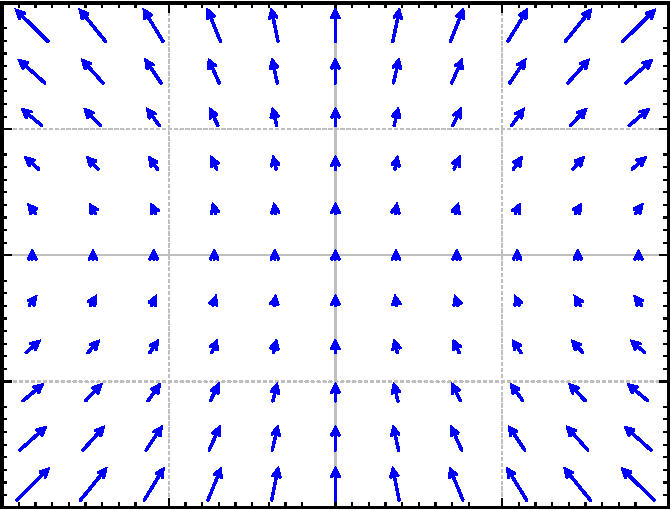
\includegraphics[width=1.75in]{figures/nlin-exer-xy-1py2}}
\task
\parbox[c]{1.75in}{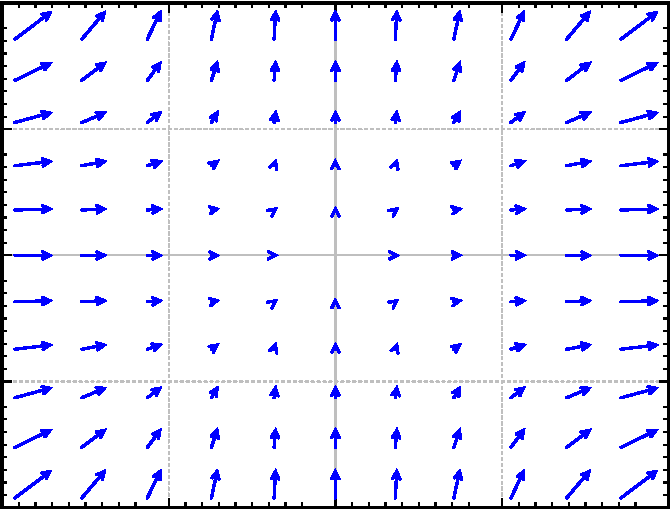
\includegraphics[width=1.75in]{figures/nlin-exer-x2-y2}}
\task
\parbox[c]{1.75in}{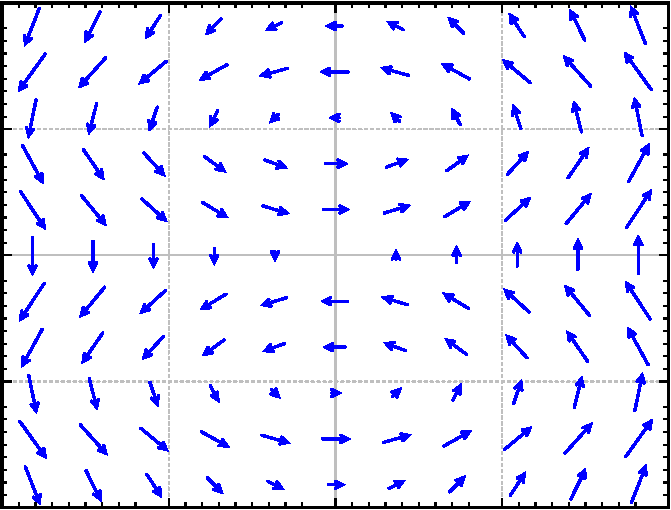
\includegraphics[width=1.75in]{figures/nlin-exer-sinpiy-x}}
\end{tasks}
\end{exercise}
\end{samepage}

\begin{exercise}\ansMark%
Match systems
\begin{equation*}
(i)\  x'=y^2, \enspace y'=-x^2, \quad (ii)\  x'=y, \enspace y'=(x-1)(x+1), \quad (iii)\  x'=y+x^2, \enspace y'=-x,
\end{equation*}
to the vector fields below.  Justify.
\begin{tasks}(3)
\task \parbox[c]{1.75in}{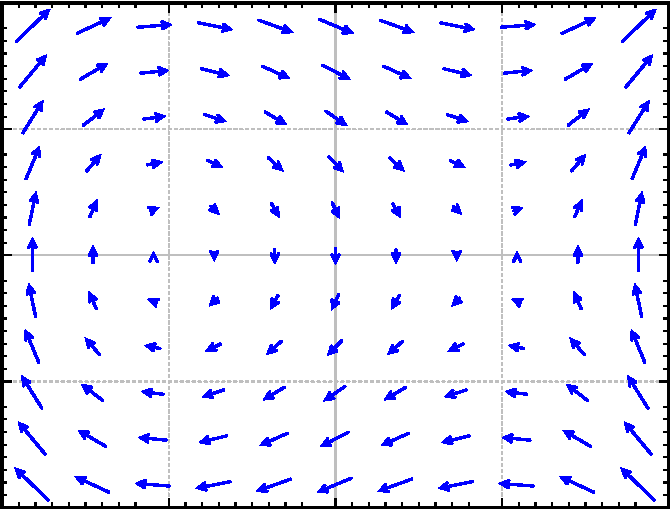
\includegraphics[width=1.75in]{figures/nlin-exer-y-xm1xp1}}
\task \parbox[c]{1.75in}{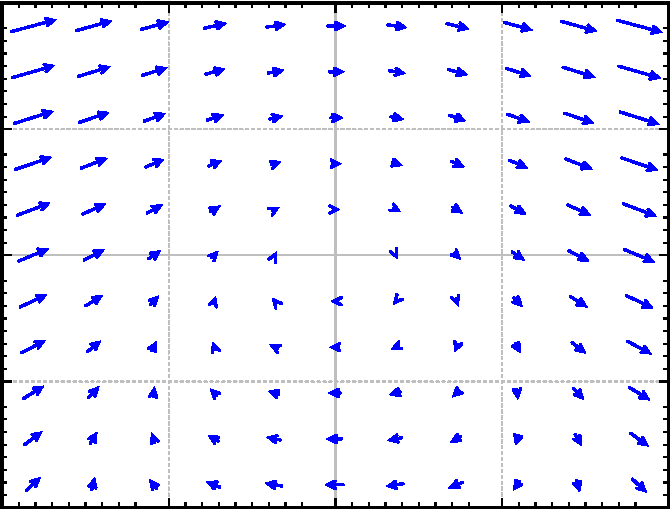
\includegraphics[width=1.75in]{figures/nlin-exer-ypx2-mx}}
\task \parbox[c]{1.75in}{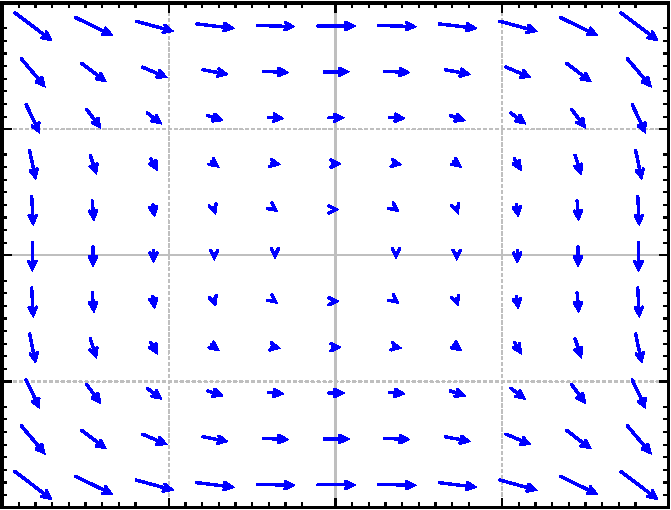
\includegraphics[width=1.75in]{figures/nlin-exer-y2-mx2}}
\end{tasks}
\end{exercise}
\exsol{%
(i) is c), \quad (ii) is a), \quad (iii) is b)
}


\begin{exercise}
Find the critical points and linearizations of the following systems.
\begin{tasks}(2)
\task $x'=x^2-y^2$, \enspace $y'=x^2+y^2-1$,
\task $x'=-y$, \enspace $y'=3x+yx^2$,
\task $x'=x^2+y$, \enspace $y'=y^2+x$.
\end{tasks}
\end{exercise}

\pagebreak[2]
\begin{exercise}\ansMark%
Find the critical points and linearizations of the following systems.
\begin{tasks}(2)
\task $x'=\sin(\pi y)+(x-1)^2$, \enspace $y'=y^2-y$,
\task $x'=x+y+y^2$, \enspace $y'=x$,
\task $x'=(x-1)^2+y$, \enspace $y'=x^2+y$.
\end{tasks}
\end{exercise}
\exsol{%
a) Critical points $(0,0)$ and $(0,1)$.  At $(0,0)$ using $u=x$, $v=y$ the linearization is $u'=-2u-(\nicefrac{1}{\pi})v$, $v'=-v$.
At $(0,1)$ using $u=x$, $v=y-1$ the linearization is
$u'=-2u+(\nicefrac{1}{\pi})v$, $v'=v$.\\
b) Critical point $(0,0)$.  Using $u=x$, $v=y$ the linearization is
$u'=u+v$, $v'=u$.\\
c) Critical point $(\nicefrac{1}{2},\nicefrac{-1}{4})$.  Using
$u=x-\nicefrac{1}{2}$, $v=y+\nicefrac{1}{4}$ the linearization is
$u'=-u+v$, $v'=u+v$.
}

\begin{exercise}
For the following systems, verify they have critical point at $(0,0)$,
and find the linearization at $(0,0)$.
\begin{tasks}(2)
\task $x'=x+2y+x^2-y^2$, \enspace $y'=2y-x^2$
\task $x'=-y$, \enspace $y'=x-y^3$
\task* $x'=ax+by+f(x,y)$, $y'=cx+dy+g(x,y)$, where
$f(0,0) = 0$,
$g(0,0) = 0$, and all first partial derivatives of $f$ and $g$ are
also zero at $(0,0)$, that is,
$\frac{\partial f}{\partial x}(0,0) = 
\frac{\partial f}{\partial y}(0,0) = 
\frac{\partial g}{\partial x}(0,0) = 
\frac{\partial g}{\partial y}(0,0) = 0$.
\end{tasks}
\end{exercise}

\begin{exercise}
Take the system $x' = (x-2)(x+y)$, \ $y' = (y+3)(x-y)$.
\begin{tasks}
\task Find all critical points.
\task Determine the linearization of this system around each of the critical points.
\task For each of the critical points, determine the behavior and classify the type of solution that the \emph{linearized} system will have around that critical point. 
\end{tasks}
\end{exercise}

\begin{exercise}
Take the system $x' = (x^2 - y)(x+3)$, \ $y' = (y-1)(x+y+1)$.
\begin{tasks}
\task Find all critical points.
\task Determine the linearization of this system around each of the critical points.
\task For each of the critical points, determine the behavior and classify the type of solution that the \emph{linearized} system will have around that critical point. 
\end{tasks}
\end{exercise}

\begin{exercise}
Take $x'=(x-y)^2$, \enspace $y'=(x+y)^2$. 
\begin{tasks}
\task Find the set of critical points.
\task Sketch a phase diagram and describe the behavior near the critical
point(s).
\task Find the linearization.  Is it helpful in understanding the system?
\end{tasks}
\end{exercise}

\begin{exercise}
Take $x'=x^2$, \enspace $y'=x^3$.
\begin{tasks}
\task Find the set of critical points.
\task Sketch a phase diagram and describe the behavior near the critical
point(s).
\task Find the linearization.  Is it helpful in understanding the system?
\end{tasks}
\end{exercise}

\begin{samepage}
\begin{exercise}\ansMark%
The idea of critical points and linearization works in higher dimensions as
well.  You simply make the Jacobian matrix bigger by adding more functions
and more variables.  For the following system
of 3 equations find the critical points and their linearizations:
\begin{equation*}
x' = x + z^2, \qquad y' = z^2-y, \qquad z' = z+x^2.
\end{equation*}
\end{exercise}
\end{samepage}
\exsol{%
Critical points are $(0,0,0)$, and
$(-1, 1, -1)$.
The linearization at the origin using variables $u=x$, $v=y$, $w=z$ is
$u' = u$, $v'=-v$, $z' = w$.
The linearization at the point $(-1,1,-1)$ using variables $u=x+1$,
$v=y-1$, $w=z+1$ is
%$x=u-1$
%$y=v+1$
%$z=w-1$
%$u' = u-1 + (w-1)^2$, $v' = (w-1)^2-v+1$, $w' = (w-1)+(u-1)^2$.
%$u' = u + w^2-2w$, $v' = w^2-2w-v$, $w' = w+u^2-2u$
$u'=u-2w$, $v'=-v-2w$, $w'=w-2u$.
}

\begin{exercise}\ansMark%
Any two-dimensional non-autonomous system $x'=f(x,y,t)$, $y'=g(x,y,t)$ can
be written as a three-dimensional autonomous system (three equations).  Write down this
autonomous system using the variables $u$, $v$, $w$.
\end{exercise}
\exsol{%
$u' = f(u,v,w)$, $v'=g(u,v,w)$, $w' = 1$.
}

\begin{exercise}
For the systems below, find and classify the critical points, also indicate
if the equilibria are stable, asymptotically stable, or unstable.
\begin{tasks}(2)
\task $x'=-x+3x^2, y'=-y$
\task $x'=x^2+y^2-1$, $y'=x$
\task $x'=ye^x$, $y'=y-x+y^2$
\end{tasks}
\end{exercise}

\begin{exercise}\ansMark%
For the systems below, find and classify the critical points.
\begin{tasks}(3)
\task $x'=-x+x^2$, $y'=y$
\task $x'=y-y^2-x$, $y'=-x$
\task $x'=xy$, $y'=x+y-1$
\end{tasks}
\end{exercise}
\exsol{%
a) $(0,0)$: saddle (unstable), $(1,0)$: source (unstable), \qquad
b) $(0,0)$: spiral sink (asymptotically stable), $(0,1)$: saddle (unstable), \qquad
c) $(1,0)$: saddle (unstable), $(0,1)$: saddle (unstable)
}

\begin{exercise}
Find and classify all critical points of the system
\[ \frac{dx}{dt} = (x+1)(x-y+3) \qquad \frac{dy}{dt} = (x-2)(x-y) .\]
\end{exercise}

\begin{exercise}
Find and classify all critical points of the system
\[ \frac{dx}{dt} = x^2 - y^2 \qquad \frac{dy}{dt} = (x+4)(y-2) .\]
\end{exercise}


\begin{exercise}
Find and classify the critical point(s) of $x' = -x^2$, $y' = -y^2$.
\end{exercise}

\begin{samepage}
\begin{exercise}
Suppose $x'=-xy$, $y'=x^2-1-y$.
\begin{tasks}
\task
Show there are two spiral sinks at
$(-1,0)$ and $(1,0)$.
\task
For any initial point of the form $(0,y_0)$, find the trajectory.
\task
Can a trajectory starting at $(x_0,y_0)$ where $x_0 > 0$ spiral into 
the critical point at $(-1,0)$?  Why or why not?
\end{tasks}
\end{exercise}
\end{samepage}

\begin{exercise} \label{exercise:increasing}
In the example $x'=y$, $y'=y^3-x$ show that for any trajectory, the distance
from the origin is an increasing function.
Conclude
that the origin behaves like is a spiral source.
Hint: Consider $f(t) =
{\bigl(x(t)\bigr)}^2 + 
{\bigl(y(t)\bigr)}^2$ and show it has positive derivative.
\end{exercise}

\begin{exercise}
Find and analyze all critical points of the system $x' = y$, $y' = -x - y^3$. Use the ideas from \exerciseref{exercise:increasing} to show that the solutions to this problem move towards the origin as $t$ grows.
\end{exercise}

\begin{exercise}\ansMark%
Derive an analogous classification of critical points for equations in one dimension,
such as $x'= f(x)$ based on the derivative.  A point $x_0$ is critical when $f(x_0) = 0$ and
almost linear if in addition $f'(x_0) \not= 0$.  Figure out if the critical point is stable or unstable
depending on the sign of $f'(x_0)$.  Explain.  Hint: see \sectionref{auteq:section}.
\end{exercise}
\exsol{%
A critical point $x_0$ is stable if $f'(x_0) < 0$ and unstable when $f'(x_0)
> 0$.
}


\setcounter{exercise}{100}

